% !TeX root = ../main.tex

\chapter{分布式文件系统中的纠删码优化}
\label{cha:design}

% 本课题采用的设计方案

\section{文件系统架构设计}
\label{sec:ch3_struct}

为了完成研究目标,本课题设计并实现了一个分布式文件系统原型。逻辑上,其结构可分为两层:文件系统层、可用性策略层。

\begin{enumerate}[(1)]
    
    \item {\heiti 文件系统层}:文件系统层处理文件系统操作逻辑。由于本课题的核心目标是证明纠删码的可行性和有效性,因此在文件系统逻辑方面,直接复用了已有的工作 LocoFS\cite{locofs2017}。LocoFS 是一个针对元数据操作进行优化的分布式文件系统原型,其逻辑简单,方便移植。LocoFS 包含三类存储节点:目录元数据服务器(DMS)、文件元数据服务器(FMS)和文件数据服务器(DS)。其中,DMS 只有一个,负责存放中心化目录元数据和进行目录操作;FMS 可以有多个,负责存放文件元数据和进行文件元数据操作;DS 有多个,负责存放文件数据。外部节点通过 LocoFS 客户端与存储集群交互,执行各种文件系统操作。
    
    \item {\heiti 可用性策略层}:可用性策略层对文件系统层提供 4KB 粒度的数据访问接口。它屏蔽底层 NVM 设备和 RDMA 通信的细节,向上层提供一个连续的虚拟 NVM 空间。当用户读写某一个虚拟页时,可用性策略层自动将其映射为对真实 NVM 设备的读写或 RDMA 访问请求。通过该层提供的抽象,只需做很少的修改,就能为文件系统应用纠删码、多副本等不同的可用性策略。

\end{enumerate}

系统的架构如图 ~\ref{fig:struct} 所示:

\begin{figure}[H]
    \centering
    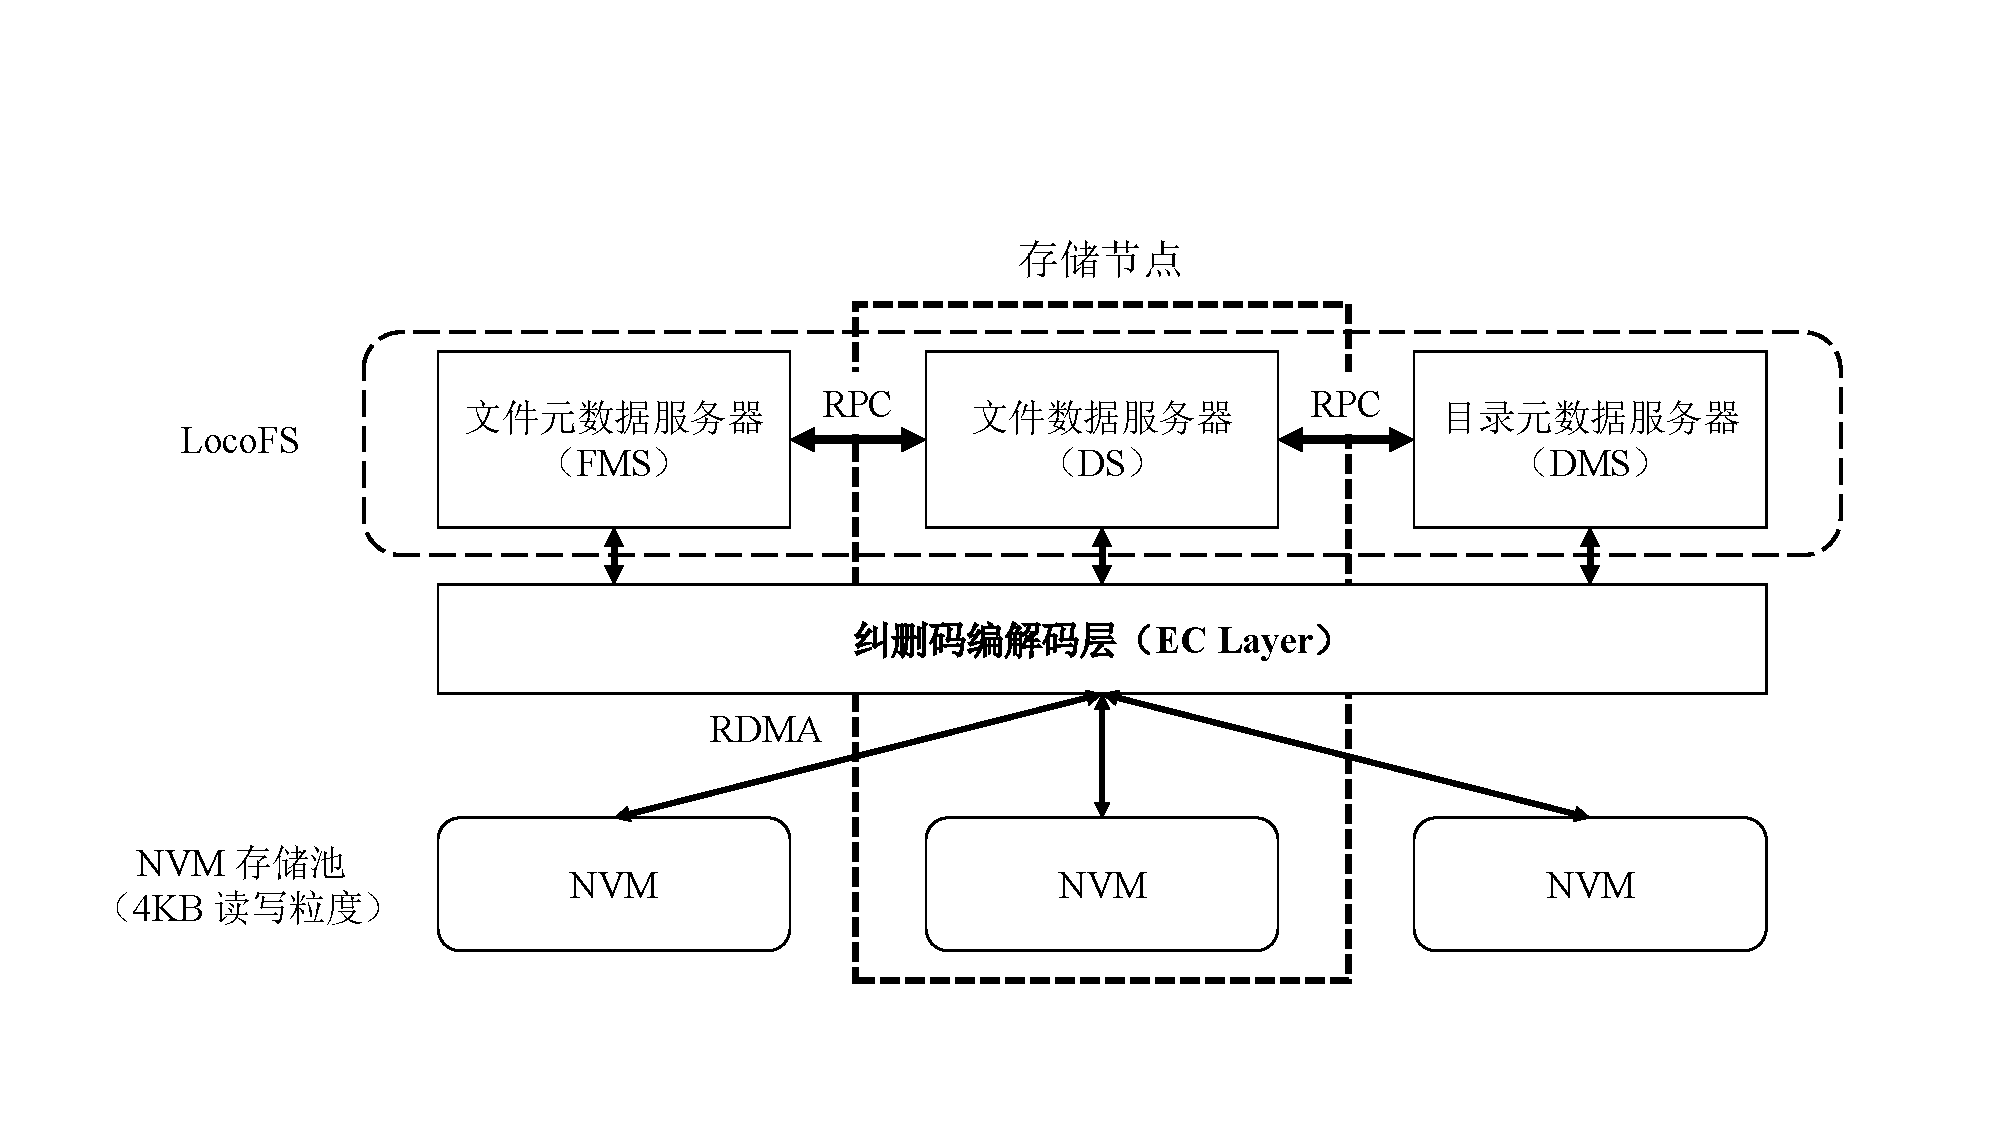
\includegraphics[width=12cm]{galois-structure.pdf}
    \caption{系统架构示意图}
    \label{fig:struct}
\end{figure}

以下各小节将详细说明文件系统的细节设计和优化方案。

\section{面向 NVM 的纠删码策略优化设计}
\label{sec:ch3_ec}

本课题中数据以 4KB 为粒度访问,每个 4KB 数据块都被独立地编码。每个 4KB 数据块被切分为 $k$ 个大小等于 $\frac{4}{k}$ KB 的编码单元,其中 $k$ 是纠删码的参数。以 $RS(4, 2)$ 为例($k = 4$),切块策略把一个 4KB 原始数据块切分为 4 个 1KB 数据块,对其编码,产生 2 个 1KB 的校验数据块,然后将 6 个 1KB 数据块分别存放于 6 个物理上分离的存储设备上。这种实现方式的优势是读写逻辑简单,并且在有节点故障的情况下,读写操作逻辑基本不受影响。

显然,相较于传统的数据备份策略,上述纠删码方案在节省存储开销方面有明显优势。在上述方案下,为了容忍任何 2 个存储节点同时发生错误,任何一个 4KB 数据块实际占用 6KB 存储空间。为了达到相同容错水平,数据备份策略需要将每个 4KB 数据块备份 2 次,合计占用 12KB 存储空间。纠删码方案节省了 50\% 的存储空间。

\subsection{朴素 Reed-Solomon 编码实现}
\label{subsec:}

如 ~\ref{subsec:ch2_avail_ec} 小节所述,Reed-Solomon 码策略 $RS(k, p)$ 需要一个 $p \times k$ 大小的列满秩矩阵 $V$。实际编码时,为了统一处理编码块将 $V$ 拼接在 $k$ 阶单位阵下方,得到一个大小为 $n \times k$($n = k + p$)的编码矩阵;编码时,用该矩阵左乘 $k$ 阶原始数据向量 $D$,得到 $p$ 阶校验和向量 $C$:
\begin{equation}
    \left(
        \begin{array}{c}
            I_{k} \\
            V
        \end{array}
    \right)
    \times
    D
    =
    \left(
        \begin{array}{c}
            D \\
            C
        \end{array}
    \right)
\end{equation}

为了编码时的简便,矩阵乘法操作通常在伽罗华域 $GF(2^8)$ 上进行。此时,加法操作变为按位异或;乘法操作虽然较为复杂,但可以利用查表法高效实现。重复执行矩阵乘法,即可实现对任意相同长度数据的编码。

在解码时,需要首先根据待解码数据的来源,取出编码矩阵中的 $k$ 行构成一个 $k$ 阶方阵,然后计算其逆矩阵。计算逆矩阵的代价随 $V$ 的选取有所不同,本课题使用了 $GF(2^8)$ 下的 Cauchy 矩阵作为 $V$,求逆只需要 $O(k^2)$ 的时间复杂度。

综合使用上述策略,就能以基本最高的效率实现朴素的 Reed-Solomon 码编解码操作。本课题据此完整地实现了任意参数的 Reed-Solomon 码编解码算法,用作其他纠删码优化方案的基线对照。使用 $RS(4, 2)$ 编码 16KB 数据进行测试,一次编码操作平均耗时 $\SI{159.2}{\us}$。显然,在高速 RDMA 网络通信环境、一次网络请求仅需数微秒的情况下,该方案效率十分低下,会让计算成为整个系统的瓶颈。

\subsection{基于 SIMD 指令集的 Reed-Solomon 编码优化}
\label{subsec:ch3_rs_simd}

我们观察到,朴素的 Reed-Solomon 码实现的运行耗时与待编码数据长度成正比,重复的矩阵乘法运算占用了大量时间。由于本课题中文件系统规定必须以 4KB 页为单位进行数据读写,待编码数据在存储上必定连续,这使我们使用单指令多数据流指令(SIMD)对编码进行优化。

Intel 的大部分 CPU 产品提供了三种 SIMD 指令集支持,分别为 SSE、AVX 和 AVX2。SSE 是 Intel 于 1999 年推出的 SIMD 指令集,支持 128 位的向量处理;AVX 是 Intel 于 2007 年推出的 SIMD 指令集,支持 256 位浮点 SIMD 运算支持;AVX2 则是于 2014 年推出的 AVX 的扩展,增加了 256 位整点 SIMD 运算支持。

Intel 在其存储加速库(Intel Storage Acceleration Library,ISA-L)中提供了开源的向量运算实现,其中就包括伽罗华域 $GF(2^8)$ 上的向量乘法和加法运算。本课题利用 ISA-L 实现了 SIMD 指令加速的纠删码编解码算法。使用 $RS(4, 2)$ 编码 16KB 数据进行测试,分别使用 SSE、AVX 和 AVX2 指令集加速,一次编码操作平均耗时分别为 $\SI{3.31}{\us}$、$\SI{2.98}{\us}$ 和 $\SI{2.37}{\us}$。

可见,SIMD 指令的引入大大降低了纠删码的编解码开销(加速比超过 50),使 NVM+RDMA 存储环境下纠删码的运用成为可能。另外也可看出,越新的指令集的运行效率也越高。因此,本课题选用 AVX2 指令集对所有纠删码操作进行加速。

\subsection{面向分布式 NVM 的 Clay Code 编码优化}
\label{subsec:ch3_claycode}

Reed-Solomon 码设计和实现简单,但有时难以满足实际需求。例如,朴素的 Reed-Solomon 码允许通过 $k$ 份存活的数据恢复其余所有 $p$ 份数据;但这同时表明任意 $k$ 份数据线性无关,在执行数据恢复时,必须首先从 $k$ 个节点中分别完整读取 1 份数据(合计 $k$ 份)。实际应用中,为了降低存储代价、提升存储效率,$k$ 的取值一般较大;因此,一个故障节点在执行恢复时将产生巨大的网络开销,有可能严重影响系统的执行效率。

不过,已有工作\cite{dimakis2010}表明,可以通过设计合适的编码方式,减少进行恢复时需要读取的数据。如果从 $d$($d \geq k$)个节点中读取数据,那么只需从每个节点中分别读取 $\frac{1}{d - k + 1}$ 份数据即可。此时总共需要读取的数据量为 $\frac{d}{d - k + 1}$ 份;显然 $\frac{d}{d - k + 1} \leq k$ 恒成立,并且当且仅当 $d = k$ 时取到等号。

Clay Code\cite{claycode2018} 是 2018 年由印度学者发表的一个 Reed-Solomon 码变种,它针对上述问题实现了最优化,同时具有设计和实现相对简单的优点。这一工作基于 Ceph 实现;由于 Ceph 使用高延迟的传统块设备作为存储介质,CPU 计算开销并系统瓶颈,因此原本的实现没有针对纠删码编解码进行优化。本课题希望评估朴素 Reed-Solomon 码以外的各种纠删码策略在 NVM+RDMA 环境下的可行性。因此,本课题选取了 Clay Code 作为非朴素纠删码策略的代表,基于 ISA-L 实现了指令集优化的 Clay Code 编解码算法。

\subsection{基于 RDMA 网络的前-k 读取策略实现}
\label{subsec:ch3_first_k}

上述设计方案中,读取每个 4KB 数据页时,总是需要从 $k$ 个不同的节点处分别读取对应的数据块进行解码。在实际运用中,出于各种无法预测的原因,总会有少数节点的响应延迟明显高于平均值,这些响应即被称作尾延迟(Tail Latency)。这时,系统就不得不等待尾延迟节点返回后再将结果返回给用户,系统性能也将受制于这些尾延迟节点。

为了降低尾延迟,我们可以回顾 Reed-Solomon 码的特性:在 $k$ 个原始数据块和计算出的 $p$ 个校验数据块中,任意读取 $k$ 个都能恢复出原始数据。由于尾延迟现象是由偶然出现的个别节点导致的,我们可以应用一个非常简单的策略来过滤掉它们:随机选择位于不同存储节点上的 $k + \Delta$ 个数据块($1 \leq \Delta \leq p$),选择其中延迟最小的 $k$ 个节点读取数据。实践中难以随时检测各个节点的访问延迟,因此我们只需同时读这 $k + \Delta$ 个数据块,在读出 $k$ 个后立即开始解码。这被称作前-k 读取策略。

由于 $\Delta$ 可以取得较小(通常为 1 或 2),并且其值基本无需随 $k$ 变化,这一优化手段只会额外占用很少的网络带宽。因此,这一策略简单、有效,并且开销很低,在已有工作中已经得到广泛应用\cite{distcache2019,infinicache2020,hydra2019}。

然而,已有工作通常基于传统 TCP/IP 网络构建,在此前提下使用该策略取得了较好的效果。本课题希望评估在 RDMA 网络环境下使用该策略的可行性和有效性,以及其对性能带来的实际改进。因此,本课题同样实现了该策略,并且为了简单起见固定取 $\Delta = 1$。

\section{可用性分析}
\label{sec:ch3_avail}

如上所述,本课题实现了两种纠删码策略,分别为朴素的 Reed-Solomon 码,及其变种 Clay Code。后者仅针对数据恢复过程进行优化,在可用性方面本质上与前者相同。因此,以下仅讨论朴素 Reed-Solomon 码 $RS(k, p)$ 的情况。

本课题直接使用了 LocoFS 的文件系统架构。如图 ~\ref{fig:struct} 所示,节点分为 DMS、FMS 和 DS 三类,这三类节点分别使用不同的可用性策略。

对于 DMS 和 FMS 而言,它们仅用于存储元数据,并且读写粒度较小。如果在其上应用纠删码会导致严重的写放大,传统的数据备份策略更加适合这种情况。由于这并非本课题的研究重点,本课题没有实现对 DMS 和 FMS 的数据备份。然而,已有工作\cite{mojim2015}早已提供了成熟的基于主从备份的解决方案,并且过往研究也证明了此方案的可行性\cite{orion2019}。采用已有研究成果,系统能容忍 DMS 和 FMS 中任意 $p$ 个节点同时故障。因此,本课题虽然不在 DMS 和 FMS 上实现相应的可用性策略,但这并不影响课题的核心结论。

对于 DS 而言,它们用于存储文件数据。本课题针对 DS 使用纠删码提供可用性保障。文件系统中所有存储文件内容的 4KB 页都经过 $RS(k, p)$ 编码,并分别存储在 $k + p$ 个节点上。在故障节点数不超过 $p$ 的情况下,对任何一个数据页的读写都能成功;故障节点在恢复后,也能通过至少 $k$ 个其他存活节点自主执行恢复数据,并在成功后重新加入存储集群。因此,系统能容忍任意 $p$ 个 DS 节点同时故障。

综上所述,系统在理论上能容忍任意 $p$ 个节点同时发生故障。
